% Tool reference on a milling spindle: support point (spindle nose) and
% registration point (tool holder), before and after mounting
\documentclass[dvisvgm,tikz,border=4pt]{standalone}
% Shared preamble for the TikZ figures in images-1/src (compiled by build.sh)
\usepackage{helvet}
\renewcommand\familydefault{\sfdefault}
\usepackage{amsmath, amssymb}
\usetikzlibrary{arrows.meta, calc, decorations.pathreplacing, patterns, positioning, shapes.geometric, 3d, perspective, fit, backgrounds}
% palette shared with slides.scss and the Graphviz diagrams
\definecolor{dmred}{HTML}{880000}
\definecolor{dmblue}{HTML}{000088}
\definecolor{dmgreen}{HTML}{008800}
\definecolor{dmorange}{HTML}{E08A1E}
\definecolor{ink}{HTML}{333333}
\definecolor{fillblue}{HTML}{E8E8F8}
\definecolor{fillred}{HTML}{F3EAEA}
\definecolor{fillgreen}{HTML}{E8F4E8}
\definecolor{fillorange}{HTML}{FDF0DC}
\definecolor{steel}{HTML}{C9D3DC}
\definecolor{steeldk}{HTML}{8FA3B5}
\definecolor{metal}{HTML}{D9D9D9}
\definecolor{metaldk}{HTML}{A6A6A6}
\tikzset{
  >={Stealth[length=7pt]},
  every picture/.style={line cap=round, line join=round, font=\large},
  proj/.style={gray, dashed, thin},
  dim/.style={<->, >={Stealth[length=5pt]}, thin},
  ext/.style={very thin, gray},
  callout/.style={gray!70!black, thin},
  % datum (origin) symbol
  % pics use absolute sizes so they look the same in mm-scaled drawings
  datum/.pic={
    \fill[white] (0,0) circle (0.22cm);
    \fill[black] (0,0) -- ++(0.22cm,0) arc[start angle=0, end angle=-90, radius=0.22cm] -- cycle;
    \fill[black] (0,0) -- ++(-0.22cm,0) arc[start angle=180, end angle=90, radius=0.22cm] -- cycle;
    \draw[thick] (0,0) circle (0.22cm);
  },
  % reference symbols (absolute sizes): origins have a double circle with a filled quadrant
  wporigin/.pic={
    \draw[thick, fill=white] (0,0) circle (0.3cm);
    \fill[black] (0,0) -- (0.18cm,0) arc[start angle=0, end angle=-90, radius=0.18cm] -- cycle;
    \draw[thick] (0,0) circle (0.18cm);
    \draw (-0.3cm,0) -- (0.3cm,0) (0,-0.3cm) -- (0,0.3cm);
  },
  machorigin/.pic={
    \draw[thick, fill=white] (0,0) circle (0.3cm);
    \fill[black] (0,0) -- (-0.18cm,0) arc[start angle=180, end angle=90, radius=0.18cm] -- cycle;
    \draw[thick] (0,0) circle (0.18cm);
    \draw (-0.3cm,0) -- (0.3cm,0) (0,-0.3cm) -- (0,0.3cm);
  },
  supportpt/.pic={
    \draw[thick, fill=white] (0,0) circle (0.15cm);
    \draw (-0.15cm,0) -- (0.15cm,0) (0,-0.15cm) -- (0,0.15cm);
  },
  regpt/.pic={
    \draw[thick, fill=white] (0,0) circle (0.24cm);
    \draw[thick] (0,0) circle (0.15cm);
    \draw (-0.15cm,0) -- (0.15cm,0) (0,-0.15cm) -- (0,0.15cm);
  },
  % support / registration point (generic)
  target/.pic={
    \draw[thick, fill=white] (0,0) circle (0.12cm);
    \draw (-0.2cm,0) -- (0.2cm,0) (0,-0.2cm) -- (0,0.2cm);
  },
}

\begin{document}
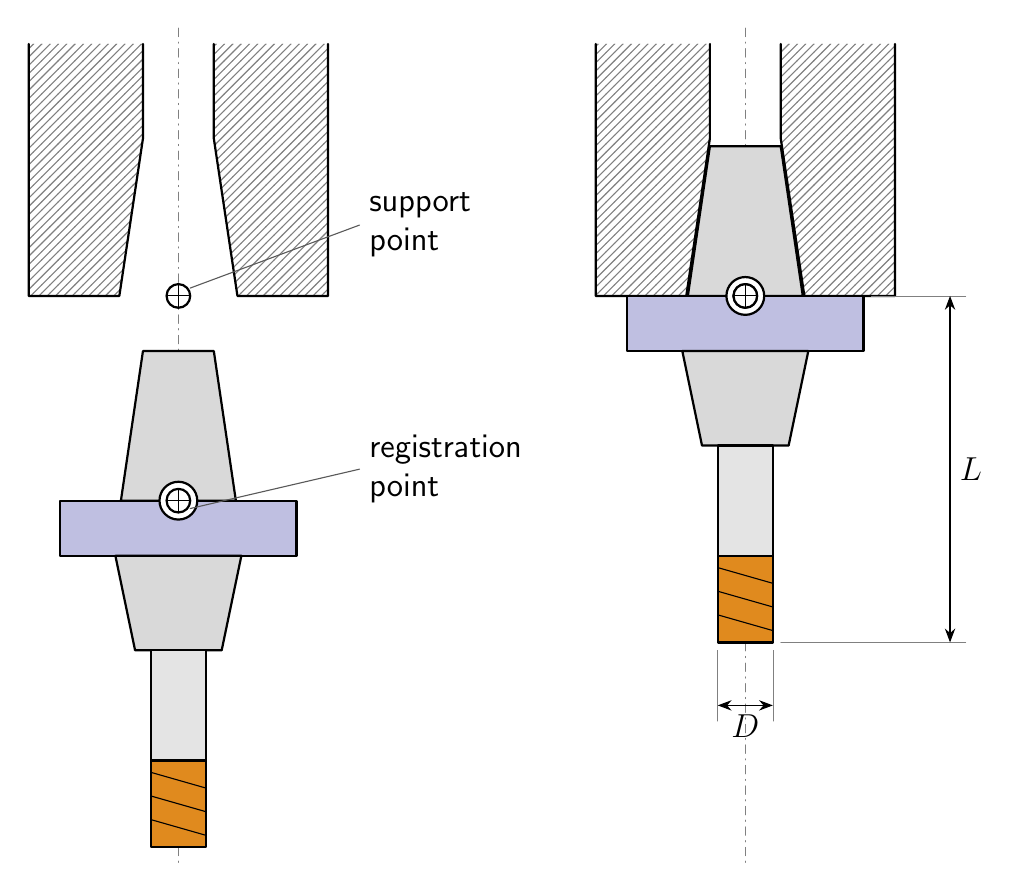
\begin{tikzpicture}[font=\large]
  % spindle nose in section, nose face at y=0, tapered bore
  \newcommand\spindle{%
    \fill[pattern=north east lines, pattern color=gray] (-1.9,0) -- (-0.75,0) -- (-0.45,2.0) -- (-0.45,3.2) -- (-1.9,3.2) -- cycle;
    \fill[pattern=north east lines, pattern color=gray] (1.9,0) -- (0.75,0) -- (0.45,2.0) -- (0.45,3.2) -- (1.9,3.2) -- cycle;
    \draw[thick] (-1.9,3.2) -- (-1.9,0) -- (-0.75,0) -- (-0.45,2.0) -- (-0.45,3.2);
    \draw[thick] (1.9,3.2) -- (1.9,0) -- (0.75,0) -- (0.45,2.0) -- (0.45,3.2);
    \draw[dash dot, gray] (0,3.4) -- (0,-7.2);
  }
  % tool holder: taper, flange (registration face at y=0), end mill
  \newcommand\holder{%
    \filldraw[thick, fill=metal] (-0.73,0) -- (-0.45,1.9) -- (0.45,1.9) -- (0.73,0) -- cycle;
    \filldraw[thick, fill=dmblue!25] (-1.5,0) rectangle (1.5,-0.7);
    \filldraw[thick, fill=metal] (-0.8,-0.7) -- (-0.55,-1.9) -- (0.55,-1.9) -- (0.8,-0.7) -- cycle;
    \filldraw[thick, fill=metal!70] (-0.35,-1.9) rectangle (0.35,-3.3);
    \filldraw[thick, fill=dmorange] (-0.35,-3.3) rectangle (0.35,-4.4);
    \foreach \y in {-3.45,-3.75,...,-4.3} \draw[thin] (-0.35,\y) -- (0.35,\y-0.2);
    \pic at (0,0) {regpt};
  }
  % ---- left: tool holder not yet mounted
  \begin{scope}
    \spindle
    \begin{scope}[yshift=-2.6cm] \holder \end{scope}
    \pic at (0,0) {supportpt};
    \draw[callout] (0.15,0.1) -- (2.3,0.9) node[right, black, align=left] {support\\point};
    \draw[callout] (0.15,-2.7) -- (2.3,-2.2) node[right, black, align=left] {registration\\point};
  \end{scope}
  % ---- right: mounted, the two points coincide
  \begin{scope}[xshift=7.2cm]
    \spindle
    \holder
    \pic at (0,0) {supportpt};
    \draw[ext] (1.6,0) -- (2.8,0) (0.45,-4.4) -- (2.8,-4.4);
    \draw[dim] (2.6,0) -- node[right] {$L$} (2.6,-4.4);
    \draw[ext] (-0.35,-4.5) -- (-0.35,-5.4) (0.35,-4.5) -- (0.35,-5.4);
    \draw[dim] (-0.35,-5.2) -- node[below] {$D$} (0.35,-5.2);
  \end{scope}
\end{tikzpicture}
\end{document}
